\section{Parallelization using the GPU}

% -------------------------------------------------------------------------------------- %

\subsection{GPU Architechture}

While parallelizing code specifically for a CPU, one wishes to increase the amount of 
instruction-level-parallelism \emph{per thread}. The CPU is built to perform tasks which 
are as large as possible, and with a little latency as possible, in a serial fashion. 
Latency is hidden on the CPU via large low-latency on-chip caches and by out-of-order 
execution. However, one could alternatively approach the problem of increasing  parallelism 
and hiding latency by increasing the number of threads entirely. This is the core core 
philosophy behind \emph{massively parallel computing} - the philosophy adopted in the GPU. 
The GPU follows a throughput-oriented design in which as many tasks as possible are 
assigned to different threads concurrently. Less focus is given to low-latency memory 
access and operations, and more focus is given to launching many separate threads. \\

To manage this amount of parallel work, the components of a GPU are split into a 
hierarchy: 

\begin{itemize}
    \item A single processing unit is known as a thread. A single consumer-level GPU can 
    have on the order of tens of thousands of threads (Compare this with the threadcount 
    of a typical consumer-level CPU of 16 or 32 threads). 
    \item Threads are grouped into warps. Each warp consists of 32 threads and a 
    \emph{warp scheduler}. This is the most granular level of scheduling that a GPU has. 
    In particular this means that every thread in a warp performs a single instruction 
    on different data. If a SIMD set (a set of data for which one operation should occur) 
    is larger than the size of a warp, then the whole warp is launched multiple times. 
    \item Threads are further grouped into (variably sized) blocks. Blocks are used by 
    the next level in the hierarchy (SM) to manage execution over the GPU.
    \item Finally, blocks are grouped into streaming multiprocessors or SMs. Each SM 
    contains an instruction register as well as a block scheduler. Instructions and data 
    which get sent to the GPU are split and stored in the SMs. Each SM can then schedule 
    tasks to the blocks that it controls. 
\end{itemize}

\begin{figure}[ht]
    \centering
    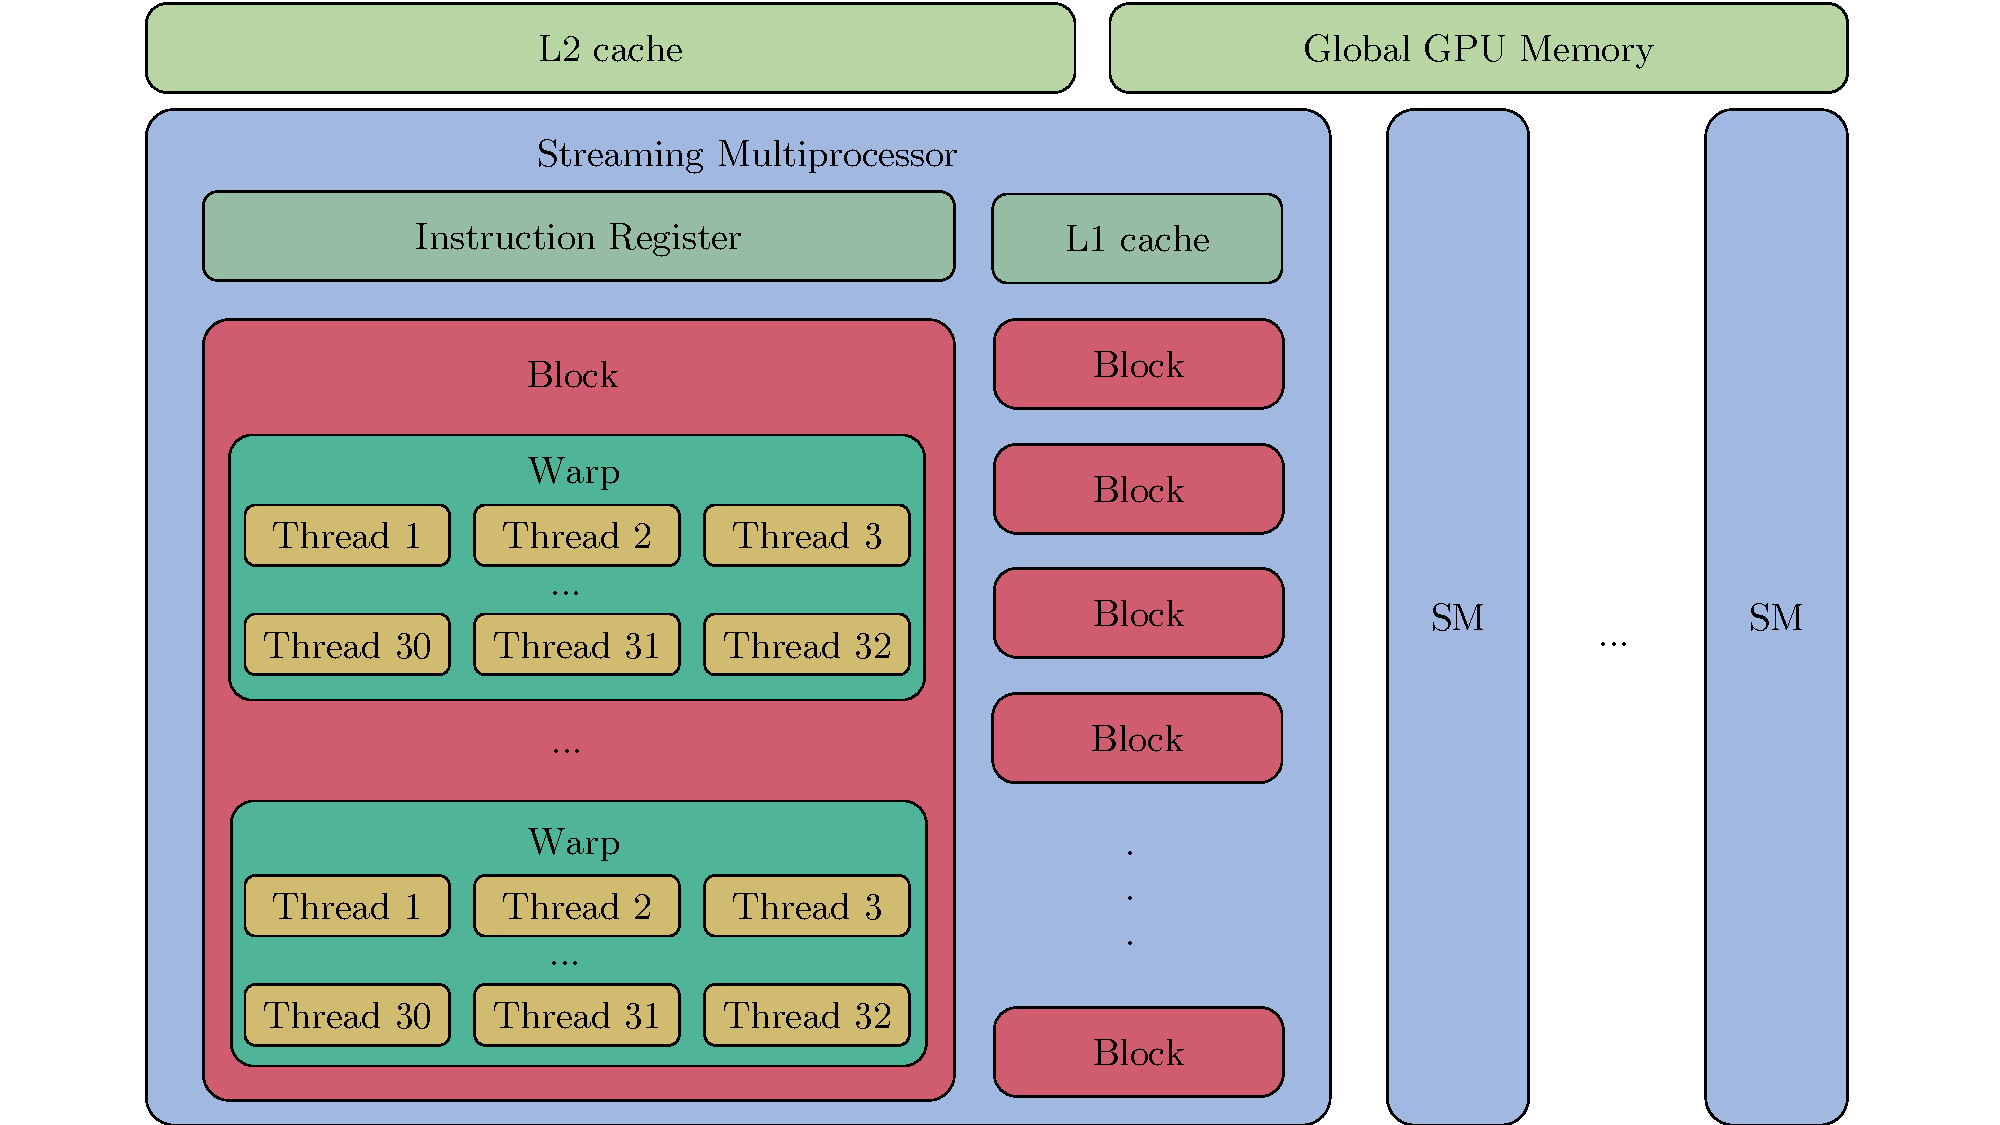
\includegraphics[width=\textwidth]{GPU_microarchitecture.pdf}
    \caption{GPU microarchitecture}
    \label{fig:gpu}
\end{figure}



% -------------------------------------------------------------------------------------- %
